\section{Семинар 6}

\begin{reminder}
    $C^*([-\pi, \pi])$~---~это все непрерывные на $[-\pi, \pi]$ функции такие, что $f(-\pi) = f(\pi)$. Норма из $C([-\pi, \pi])$
\end{reminder}

\begin{problem}
    Полна ли система $T = \{1, \cos{x}, \sin{x}, \ldots, \cos{nx}, \sin{nx}, \ldots\}$ в пространстве $C^*([-\pi, \pi])$?
\end{problem}

\begin{solution}
    Да, по теореме Фейера.
\end{solution}

\begin{problem}
    Полна ли система $K = \{1, \cos{x}, \cos{2x}, \ldots, \cos{nx}, \ldots\}$ в пространстве $C^*([-\pi, \pi])$?
\end{problem}

\begin{solution}
    Нет, не полна.\\
    Рассмотрим $f(x) = \sin{x}$, её нельзя приблизить никакой линейной комбинацией из системы K. Действительно, пусть $P_n (x) = \sum_{k = 0}^n a_k \cos{kx}$. Тогда надо показать, что
    $$A = \sup_{x \in [-\pi / 2, \pi / 2]}|\sin{x} - P_n(x)| \geq \text{const (не зависящей от выбора } P_n).$$
    Понятно, что супремум по большему множеству не меньше, чем по меньшему. Тогда $$A \geq \max\{|\sin{(\pi / 2)} - P_n(\pi / 2)|, |\sin{(-\pi / 2)} - P_n(-\pi / 2)|\}.$$
    Но в силу четности косинуса $P_n(\pi / 2) = P_n(-\pi / 2).$ Итак, $A \geq \{ |1 - P_n(\pi / 2)|, |-1 - P_n(\pi / 2)| \}$.
    Далее заметим, что
    $$|2| \leq |1 \pm P_n (x) + 1| \leq |1 - P_n (x)| + |1 + P_n (x)| \leq 2 \max\{\ldots\} \Longrightarrow A \geq 1.$$

    Итого мы показали, что нужно.
\end{solution}

\begin{problem}
    Рассмотрим подпространство E пространства $C([0, \pi / 2])$, состоящее из функций $f(0) = 0$. Доказать, что система $\{ \sin{x}, \sin{3x}, \ldots, \sin{(2n + 1), \ldots\}}$ полна в E.
\end{problem}

\begin{solution}
    Заметим, что $\sin{\left((2n + 1) (\pi / 2 - \alpha)\right)} = \sin{\left((2n + 1) (\pi / 2 + \alpha)\right)} \ \forall \alpha \in (0, \pi / 2)$.
    \begin{enumerate}
        \item Четно продолжим $f$ относительно прямой $x = \pi / 2$ (имеется ввиду, что если рассмотреть ограничение графика на $[0, \pi]$, то он будет симметричен относительно нее и выполняться свойство выше);
        \item Далее то, что получилось, продолжим нечетно относительно начала координат;
        \item И наконец, продолжим $2\pi$-периодично.
    \end{enumerate}
    \begin{figure}[h!]
\begin{center}
    \begin{minipage}[h]{0.45\linewidth}
    \centering
    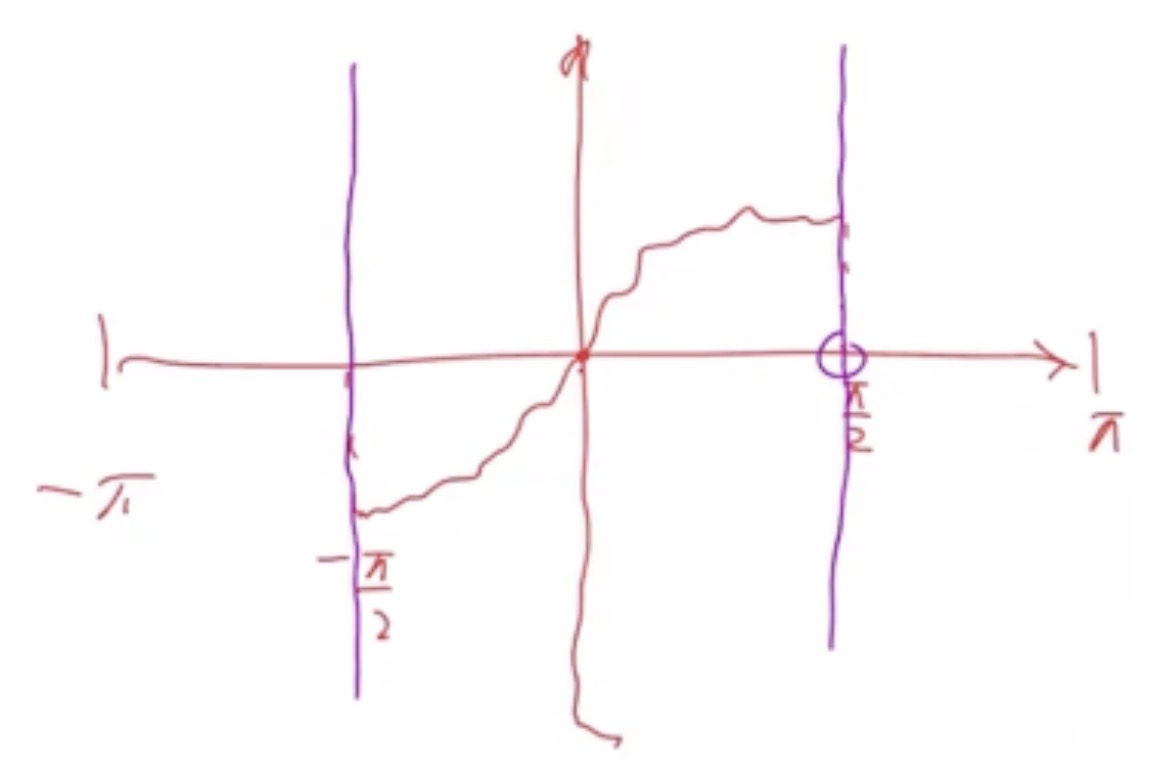
\includegraphics[width=8cm]{Pictures/sem6_1.jpeg}
    \end{minipage}
    \hfill
    \begin{minipage}[h]{0.45\linewidth}
    \begin{center}
        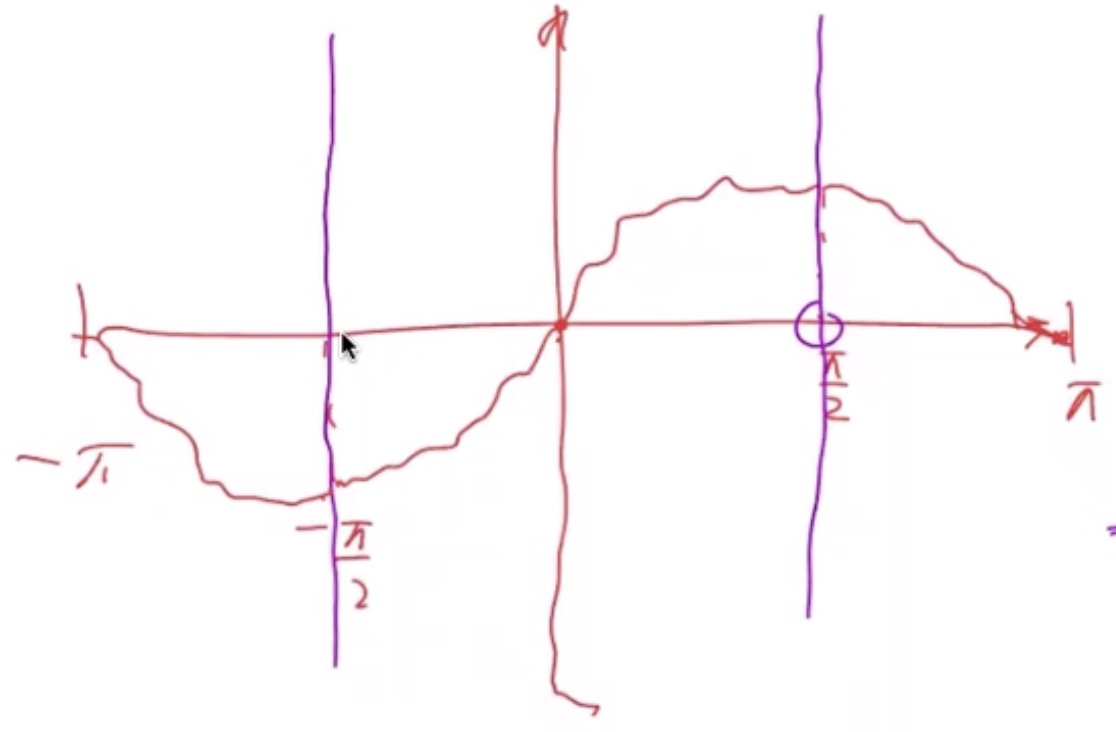
\includegraphics[width=8cm]{Pictures/sem6_2.jpeg}
    \end{center}
    \end{minipage}
    \hfill

\end{center}
\end{figure}
    Вспомним, что сумма Фейера $\displaystyle \sigma_n [f] = \cfrac{1}{n} \sum_{k = 0}^{n - 1} S_k [f]$, а в суммы Фурье, ввиду созданной нами симметрии, будут стоять ненулевые коэффициенты только при $\sin{(2k + 1) x}, \ \forall k \in \mathbb{N}$ (при косинусах они будут 0 засчет нечетности, а при <<четных синусах>>, то есть $\sin{(2k)x}$, засчет созданной нами симметрии).

    А далее по теореме Фейера получаем искомое.
\end{solution}

\subsection{Пространства $l_p$}

\begin{definition}
    Пространство $\displaystyle l_p := \left\{ x = (x_1, x_2, \ldots, x_n, \ldots) : \sum_{k = 1}^{+\infty} |x_k|^p < +\infty \right\},$ $p \in [1, +\infty)$.\\
    Норма $\displaystyle \| x\|_p := \left( \sum_{k = 1}^{+\infty} |x_k|^p \right)^{1 / p}$.

    По определению $l_{\infty}$~---~линейное пространство всех ограниченных последовательностей с нормой $\displaystyle \| x\|_{\infty} := \sup_{k \in \mathbb{N}} |x_k|$.
\end{definition}

\begin{note}
    Заметим, что $l_p \subset l_q$, где $1 \leq p \leq q \leq +\infty$.

    Интуитивно это можно запомнить с помощью: $l_{\infty}$~---~самое широкое, $l_1$~---~самое узкое.
\end{note}

\begin{remark}
    Строго говоря, для этого надо доказать неравенство
    $$\left( \sum_{k = 1}^{\infty} |x_k|^p\right)^{1/p} \geq \left( \sum_{k = 1}^{\infty} |x_k|^q\right)^{1/q}, \quad 1 \leq p \leq q.$$
\end{remark}

\begin{definition}
    Множество E в метрическом пространстве $X = (X, \rho)$ называется всюду плотным, если его замыкание совпадает со всем пространством.
\end{definition}

\begin{definition}
    $C_{00}$~---~пространство всех финитных последовательностей, то есть
    $$x \in C_{00} \Longleftrightarrow \exists N(x) \in \mathbb{N}\text{: } x_n = 0 \ \forall n \geq N(x).$$
\end{definition}

\begin{problem}
    Доказать, что $l_1$ всюду плотно в $l_2$.
\end{problem}

\begin{solution}
    Покажем, что $C_{00}$~---~плотно в $l_p$ $\forall p \in [1, +\infty)$. Отсюда сразу будет следовать требуемое, так как очевидно $C_{00} \subset l_p \ \forall p \geq 1$ (в частности $C_{00} \subset l_1$) и если $\overline{C_{00}} = l_p \ \forall p \in [1, +\infty)$, то получаем $\overline{l_1} = l_p \ \forall p \in [1, +\infty)$.

    Пусть $x \in l_p$. Тогда
    \begin{multline*}
        \forall \epsilon > 0 \ \exists N(\epsilon): \left( \sum_{k = N(\epsilon) +1}^{\infty} |x_k|^p\right)^{1/p} < \epsilon \Longrightarrow  \forall \epsilon > 0 \  \exists x_{\epsilon}= (x_1, \ldots, x_{N(\epsilon)}, 0, \ldots, 0, \ldots) \in C_{00}: \\ \|x - x_{\epsilon}\|_p = \left( \sum_{k = 1}^{\infty} |x_k - (x_{\epsilon})_k|^p\right)^{1/p} = \left( \sum_{k = N(\epsilon) +1}^{\infty} |x_k|^p\right)^{1/p} < \epsilon.
    \end{multline*}
    Итого мы получаем, что нужно, как следствие.
\end{solution}

\begin{problem}
    (Задача была на отл, гойда)
\end{problem}

\newpage
\subsection{Аппроксимативная единица (метод сглаживания)}

\begin{definition}
    Семейство функций $\{ w_t\}_{t > 0} \subset C(\mathbb{R}^n)$ называется аппроксимативной единицей, если
    \begin{enumerate}
        \item $w_t (x) \geq 0$ $\forall x \in \mathbb{R^n}$ $\forall t > 0$;
        \item $\displaystyle \forall t > 0 \hookrightarrow \int_{\mathbb{R^n}} w_t(x), \text{d} x = 1$;
        \item фокусирующее свойство:
        $$\forall \delta > 0 \ \lim_{t \to + 0} \int_{\mathbb{R^n} \backslash B_{\delta} (0)} w_t (x) \text{d} x = 0.$$
    \end{enumerate}
\end{definition}


\begin{example}
    Соболевская шапочка:
    $$\varphi(x) = \begin{cases}
        e\cdot e^{-\frac{1}{(x-1)^2}}, \ |x| < 1 \\
        0, \ |x| \geq 1
    \end{cases}$$
    $\varphi(x) \in C_{0}^{\infty} (\mathbb{R^n})$, $\displaystyle \int_{\mathbb{R^n}} \varphi(x) \text{d} x = 1$ (вообще говоря, это какая-то константа, но можно отнормировать на единицу).

    Далее рассмотрим $\varphi_{\epsilon} (x) = \cfrac{1}{\epsilon^n} \varphi\left( \cfrac{x}{\epsilon}\right)$. Тогда $\{ \varphi_{\epsilon} \}_{\epsilon > 0}$~---~аппроксимативная единица.

\end{example}